% ==============================================================================
% فصل ششم: پردازش و رمزگشایی Trace
% ==============================================================================

\chapter{پردازش و رمزگشایی \lr{Trace}}
\label{ch:decoding}

\section{مقدمه}
داده‌های دیجیتال خام ثبت‌شده بر روی حافظه لاجیک‌آنالایزر، دنباله‌ای از نمونه‌های ولتاژ ناهمگام هستند که بدون طی یک خط‌لوله پردازش نرم‌افزاری، فاقد معنای محاسباتی می‌باشند. پروتکل فشرده‌سازی \lr{ETMv4} یک جریان کاملاً غیرخطی از تصمیمات انشعاب و رویدادهای سیستمی است که باید با کدهای باینری فایل کامپایل‌شده (\lr{ELF}) تلفیق شود تا به دستورات متوالی زبان اسمبلی و زمان‌بندی دقیق تبدیل گردد. برای تحقق این هدف، اسکریپت پیشرفته پایتون موسوم به \lr{\texttt{TraceStreamProcessor.py}} طراحی و پیاده‌سازی شد. این ابزار به عنوان موتور اصلی پیش‌پردازش، وظیفه استخراج بایت‌های فریم پورت \lr{TPIU}، اعتبارسنجی یکپارچگی سیگنال‌ها، ساختاربندی اسنپ‌شات استاندارد و ادغام با موتور مرجع صنعتی \lr{OpenCSD} را بر عهده دارد. در این فصل، کالبدشکافی خط‌لوله پردازش داده، ساختار فایل‌های اسنپ‌شات، پیوند عمیق پارامترهای دکودر با ثبّات‌های سخت‌افزاری پردازنده، و در نهایت طراحی و پیاده‌سازی افزونه اختصاصی محیط توسعه \lr{VS Code} موسوم به \lr{CoreSight Trace Studio} جهت اتوماسیون کامل این فرآیندها تشریح می‌گردد.

\section[معماری اسکریپت پردازش داده \lr{TraceStreamProcessor.py}]{معماری اسکریپت پردازش داده\\ (\lr{TraceStreamProcessor.py})}
\label{sec:tracestreamprocessor_arch}
اسکریپت \lr{\texttt{TraceStreamProcessor.py}} به عنوان پل ارتباطی هوشمند میان لایه سخت‌افزار ثبت سیگنال و موتور نرم‌افزاری رمزگشای مرجع \lr{OpenCSD} عمل می‌کند. در رویکردهای اولیه، رمزگشایی مستقیم داده‌های خام با خطاهای متعددی نظیر عدم تراز فاز، گم‌شدن مرز فریم‌ها و ناسازگاری قالب مواجه می‌شد. برای غلبه بر این مسائل، خط‌لوله‌ای هفت‌مرحله‌ای و کاملاً خودکار پیاده‌سازی گردید که وظایف تبدیل، ترازسازی، اعتبارسنجی و بسته‌بندی را انجام می‌دهد. شکل \ref{fig:tracestreamprocessor_flow} فلوچارت مراحل اجرایی این اسکریپت را به تصویر کشیده است.

\begin{figure}[H]
\centering
\begin{latin}
\begin{tikzpicture}[
    node distance=0.42cm,
    stepb/.style={rectangle, draw=blue!80, fill=blue!5, thick, rounded corners=4pt, text width=13.2cm, align=center, inner sep=4pt},
    arr/.style={-latex, very thick, draw=black!70}
]
    \node [stepb] (s1) {\textbf{\rl{گام ۱: فراخوانی فایل نمونه‌های خام لاجیک‌آنالایزر}}\\[0.05cm]\small \rl{خواندن فایل} \lr{CSV} \rl{شامل نمونه‌های زمانی} \lr{TRACECLK} \rl{و ۴ خط داده} \lr{TRACED0..3}};
    
    \node [stepb, below=0.42cm of s1] (s2) {\textbf{\rl{گام ۲: آشکارسازی لبه‌های کلاک و فیلترینگ جهش‌ها (\lr{Glitch Filtering})}}\\[0.05cm]\small \rl{تشخیص لبه‌های معتبر کلاک، استخراج نیبل‌های ۴ بیتی و حذف نویز با پایدارسازی نمونه‌ها}};
    
    \node [stepb, below=0.42cm of s2] (s3) {\textbf{\rl{گام ۳: ترکیب نیبل‌ها و بازسازی بایت‌های فریم \lr{TPIU}}}\\[0.05cm]\small \rl{جفت‌سازی نیبل کم‌ارزش و پرارزش جهت تشکیل بایت‌های متوالی پروتکل سیم}};
    
    \node [stepb, below=0.42cm of s3] (s4) {\textbf{\rl{گام ۴: اعتبارسنجی فریم‌ها، ترازسازی بر پایه \lr{FSYNC} و حذف قطعات ناقص}}\\[0.05cm]\small \rl{بررسی دوره‌ای الگوهای} \lr{FSYNC/HSYNC}\rl{، رتبه‌بندی تراز فاز با بسته‌های} \lr{A-Sync}\rl{، و ترازسازی ۱۶ بایتی}};
    
    \node [stepb, below=0.42cm of s4] (s5) {\textbf{\rl{گام ۵: تفکیک سگمنت‌های بارگذاری (\lr{PT\_LOAD}) از باینری \lr{ELF}}}\\[0.05cm]\small \rl{پارس ساختار باینری ۳۲ بیتی، استخراج محتوای حافظه فلش و تولید فایل‌های دامپ} \texttt{mem\_*.bin}};
    
    \node [stepb, below=0.42cm of s5] (s6) {\textbf{\rl{گام ۶: ساختاربندی خودکار بسته اسنپ‌شات استاندارد \lr{OpenCSD}}}\\[0.05cm]\small \rl{تولید فایل‌های پیکربندی} \texttt{snapshot.ini}\rl{،} \texttt{device1.ini}\rl{،} \texttt{device2.ini} \rl{و} \texttt{trace.ini}};
    
    \node [stepb, below=0.42cm of s6] (s7) {\textbf{\rl{گام ۷: فراخوانی موتور رمزگشای \lr{trc\_pkt\_lister} و استخراج لاگ دستورات}}\\[0.05cm]\small \rl{رمزگشایی چرخه‌دقیق دستورالعمل‌ها، تفکیک روتین‌های وقفه، و محاسبه زمان اجرای بدترین شرایط (\lr{WCET})}};

    \draw [arr] (s1) -- (s2);
    \draw [arr] (s2) -- (s3);
    \draw [arr] (s3) -- (s4);
    \draw [arr] (s4) -- (s5);
    \draw [arr] (s5) -- (s6);
    \draw [arr] (s6) -- (s7);
\end{tikzpicture}
\end{latin}
\caption{فلوچارت خط‌لوله پردازش هفت‌مرحله‌ای اسکریپت \lr{\texttt{TraceStreamProcessor.py}}}
\label{fig:tracestreamprocessor_flow}
\end{figure}

\section[کالبدشکافی فنی مراحل پردازش در \lr{TraceStreamProcessor}]{کالبدشکافی فنی مراحل پردازش در\\ \lr{TraceStreamProcessor}}
\label{sec:processing_stages_deepdive}

\subsection{آشکارسازی لبه، حذف گلیچ و استخراج نیبل‌ها}
در مد ردیابی موازی ۴ بیتی، هر بایت داده شامل دو نیبل ۴ بیتی است که در لبه‌های کلاک پورت \lr{TPIU} صادر می‌شوند. سیگنال‌های دریافتی از لاجیک‌آنالایزر با نرخ اورسمپلینگ ۱۰ برابری ثبت شده‌اند؛ بنابراین هر دوره تناوب کلاک با چندین نمونه دیجیتال نشان داده می‌شود. اسکریپت برای ممانعت از خطاهای ناشی از نویزهای ضربه‌ای و جهش‌های ولتاژی (\lr{Glitches})، از یک مکانیزم فیلترینگ پایداری لبه استفاده می‌کند: یک نیبل تنها زمانی معتبر شناخته می‌شود که وضعیت کلاک نسبت به نمونه پیشین تغییر کرده و برای حداقل یک نمونه در وضعیت جدید پایدار بماند. قطعه‌کد \ref{lst:nibble_extraction} پیاده‌سازی این منطق را نشان می‌دهد:

\begin{latin}
\begin{lstlisting}[language=Python, caption={\rl{منطق آشکارسازی لبه کلاک و استخراج نیبل‌ها در} \lr{\texttt{TraceStreamProcessor.py}}}, label={lst:nibble_extraction}]
def nibbles_from_csv(path):
    """
    Recover TRACEDATA nibbles from DSLogic oversampled CSV export.
    Rejects single-sample glitches by ensuring the clock state
    persists after an edge transition.
    """
    CLK_COL, D0_COL, D1_COL, D2_COL, D3_COL = 1, 2, 3, 4, 5
    nibbles = bytearray()
    prev_raw_clk = None

    with open(path, "r") as f_in:
        for row in csv.reader(f_in):
            if not row or row[0].startswith(";") or "Time" in row[0]:
                continue
            try:
                raw_clk = int(row[CLK_COL])
                nib = ((int(row[D3_COL]) << 3) | (int(row[D2_COL]) << 2) |
                       (int(row[D1_COL]) << 1) | int(row[D0_COL]))
            except (ValueError, IndexError):
                continue

            if prev_raw_clk is None:
                prev_raw_clk = raw_clk
                continue

            # Clock edge detected
            if raw_clk != prev_raw_clk:
                nibbles.append(nib)
                prev_raw_clk = raw_clk

    return nibbles
\end{lstlisting}
\end{latin}

\subsection{ترازسازی فریم‌های پروتکل \lr{TPIU} بر پایه الگوهای \lr{FSYNC}}
در استاندارد معماری \lr{CoreSight}، بایت‌های ردیابی مستقیماً به صورت خام بر روی سیم منتشر نمی‌شوند؛ بلکه در قالب فریم‌های ۱۶ بایتی پروتکل واسط پورت \lr{TPIU} بسته‌بندی می‌گردند. در این فریم‌ها:
\begin{itemize}
    \item بایت پانزدهم (بایت آخر) به عنوان بایت کمکی (\lr{Auxiliary Byte}) عمل می‌کند که بیت‌های کم‌ارزش بایت‌های زوج و نشانگرهای تغییر شناسه جریان (\lr{ATB ID}) را در خود جای داده است.
    \item برای همگام‌سازی فریم‌ها، الگوهای ویژه \lr{FSYNC} با توالی هگزادسیمال \lr{\texttt{0x7FFFFFFF}} (۴ بایت: \texttt{FF FF FF 7F}) به طور منظم در جریان داده ارسال می‌شوند. همچنین در زمان‌های بیکاری پورت، بایت‌های پرکننده \lr{HSYNC} با مقدار \lr{\texttt{0x7FFF}} (۲ بایت: \texttt{FF 7F}) درج می‌گردند.
\end{itemize}

یکی از دستاوردهای برجسته اسکریپت \lr{\texttt{TraceStreamProcessor.py}}، کشف این حقیقت مهندسی بود که \textbf{بایت‌های سیم نباید پیش از ارسال به \lr{OpenCSD} به‌صورت دستی دی‌فریم (\lr{De-frame}) شوند!} در نسخه‌های ابتدایی، اسکریپت سعی در حذف دستی بایت‌های همگام‌سازی و جداسازی بایت‌های داده داشت که به دلیل لغزش فاز موجب خطای غیرقابل‌رفع \lr{I\_BAD\_SEQUENCE} در موتور دکودر می‌شد. در نسخه توسعه‌یافته حاضر، بایت‌های کامل سیم همراه با الگوهای همگام‌سازی در قالب فایل باینری \lr{\texttt{tpiu\_wire.bin}} حفظ شده و با تعریف فرمت \lr{\texttt{coresight}} در فایل پیکربندی، دی‌فریم کردن و تطبیق فاز به دی‌فرمتور داخلی و بهینه‌شده موتور \lr{OpenCSD} واگذار می‌گردد. اسکریپت با اسکن الگوهای \lr{FSYNC}، ابتدای بافر را به نخستین فریم معتبر ۱۶ بایتی تراز کرده و قطعات ناقص ضبط اولیه و انتهایی را پیراست (\lr{Trim}) می‌نماید.

\subsection{تفکیک خودکار سگمنت‌های اجرایی باینری (\lr{ELF Reader})}
موتور رمزگشای \lr{OpenCSD} برای اینکه بتواند بسته‌های ردگیری (شامل تصمیمات انشعاب شرطی) را به کدهای اسمبلی تبدیل کند، نیازمند دسترسی به تصویر کدهای باینری موجود در حافظه فلش میکروکنترلر است. اسکریپت \lr{\texttt{TraceStreamProcessor.py}} دارای یک ماژول مستقل پارسر فایل‌های باینری \lr{ELF} ۳۲ بیتی با فرمت لیتل‌اندیان (\lr{Little-Endian}) است که بدون وابستگی به تولچین‌های سنگین خارجی (نظیر \lr{arm-none-eabi-objcopy})، مستقیماً هدرهای برنامه (\lr{Program Headers}) را کاوش نموده و سگمنت‌های با فلگ \lr{\texttt{PT\_LOAD}} را که حاوی کدهای اجرایی برنامه کاربر هستند استخراج می‌کند. محتوای این سگمنت‌ها به عنوان فایل‌های دامپ حافظه (نظیر \lr{\texttt{mem\_08000000.bin}}) در پوشه اسنپ‌شات ذخیره می‌شوند.

\section{ادغام با موتور رمزگشای مرجع \lr{OpenCSD}}
\label{sec:opencsd_integration}
پس از ایجاد و ساختاربندی پوشه اسنپ‌شات، اسکریپت ابزار خط فرمان استاندارد \lr{trc\_pkt\_lister} متعلق به بنیاد \lr{Linaro} را با دستور زیر فراخوانی می‌کند:

\begin{latin}
\begin{lstlisting}[language=bash]
trc_pkt_lister -ss_dir ./snapshot/ -tpiu_hsync -decode -logstdout \
               -o decoded_trace.txt
\end{lstlisting}
\end{latin}

در این دستور، فلگ \lr{\texttt{-tpiu\_hsync}} دی‌فرمتور سخت‌افزاری \lr{OpenCSD} را فعال می‌سازد تا بسته‌های پرکننده همگام‌سازی را حذف نماید و آرگومان \lr{\texttt{-decode}} دستور می‌دهد که کدهای باینری با جریان ردگیری تلفیق شده و دستور به دستور بازسازی گردند. عملیات دکود در سه لایه پردازشی انجام می‌گیرد:
\begin{enumerate}
    \item \textbf{پردازشگر بسته‌ها (\lr{Packet Processor}):} بایت‌های ورودی را به عناصر سازنده پروتکل \lr{ETMv4} شامل بسته‌های همگام‌سازی (\lr{I\_SYNC})، بسته‌های اتم (\lr{ATOM})، برچسب زمانی (\lr{TIMESTAMP})، شمارش چرخه (\lr{CYCLE\_COUNT}) و استثناها (\lr{EXCEPTION}) تجزیه می‌کند.
    \item \textbf{رمزگشای دستورات (\lr{Instruction Decoder}):} با استخراج نشانی شروع برنامه از بسته \lr{I\_SYNC}، کدهای ماشین را در سگمنت‌های بارگذاری‌شده دنبال می‌کند. با برخورد به دستورات انشعاب شرطی، وضعیت شاخه را از بیت‌های بسته اتم خوانده و مسیر واقعی اجرای برنامه را بازسازی می‌نماید.
    \item \textbf{قالب‌بندی عناصر ردگیری (\lr{Trace Element Formatter}):} جریان زمانی دستورات را همراه با نشانی دستور، کد اسمبلی، نام تابع مبدأ، شماره خط در کد مبدأ و شماره چرخه ماشین در قالب فایل متنی ساختاریافته استخراج می‌کند.
\end{enumerate}

\section{کالبدشکافی ساختار فایل‌های اسنپ‌شات \lr{OpenCSD}}
\label{sec:snapshot_structure}

\subsection{ساختار و محتوای فایل‌های پوشه اسنپ‌شات}
پوشه اسنپ‌شات تولیدشده توسط \lr{\texttt{TraceStreamProcessor.py}} یک کپسول کاملاً مستقل و خودکفا از شرایط تست، اتصالات سخت‌افزاری و جریان داده‌هاست. این پوشه شامل پنج جزء کلیدی است:

\paragraph*{۱. فایل پیکربندی ریشه (\lr{\texttt{snapshot.ini}}):}
این فایل به عنوان مانیفست اصلی دکودر عمل کرده و مشخصات نسخه پروتکل، اسامی فایل‌های توصیف تجهیزات و فایل متادیتای بافر را تعیین می‌کند:
\begin{latin}
\begin{lstlisting}[language=make, caption={\rl{محتوای فایل مانیفست ریشه} \lr{\texttt{snapshot.ini}}}]
[snapshot]
version=1.0

[device_list]
device1=device1.ini
device2=device2.ini

[trace]
metadata=trace.ini
\end{lstlisting}
\end{latin}

\paragraph*{۲. فایل توصیف هسته پردازنده (\lr{\texttt{device1.ini}}):}
این فایل معماری هسته پردازنده، وضعیت اولیه ثبّات‌های کنترلی آن، و ارجاع به قطعات استخراج‌شده از حافظه فلش فایل \lr{ELF} برنامه را تعریف می‌نماید:
\begin{latin}
\begin{lstlisting}[language=make, caption={\rl{محتوای فایل توصیف هسته} \lr{\texttt{device1.ini}}}]
[device]
name=Cortex-M7_0
class=core
type=Cortex-M7

[regs]
PC=0x08000000
xPSR=0x01000000

[dump1]
file=mem_08000000.bin
address=0x08000000
length=0x1E4A0
\end{lstlisting}
\end{latin}

\paragraph*{۳. فایل توصیف منبع ردگیری و ثبّات‌های سخت‌افزاری (\lr{\texttt{device2.ini}}):}
این فایل هویت منبع ردگیری را با نام \lr{\texttt{CSETM\_0}} و کلاس \lr{\texttt{trace\_source}} تعیین کرده و حیاتی‌ترین اطلاعات مورد نیاز دکودر یعنی \textbf{مقادیر ثبّات‌های سخت‌افزاری ماژول \lr{ETM}} را در خود جای داده است:
\begin{latin}
\begin{lstlisting}[language=make, caption={\rl{محتوای فایل منبع ردگیری و ثبّات‌های سخت‌افزاری} \lr{\texttt{device2.ini}}}]
[device]
name=CSETM_0
class=trace_source
type=ETM4.0

[regs]
TRCCONFIGR(0x4)=0x00000811
TRCEVENTCTL0R(0x8)=0x00000000
TRCEVENTCTL1R(0x9)=0x00000000
TRCSTALLCTLR(0xB)=0x00000000
TRCTSCTLR(0xC)=0x00000000
TRCSYNCPR(0xD)=0x0000000A
TRCCCCTLR(0xE)=0x00000040
TRCTRACEIDR(0x10)=0x0000003E
TRCVICTLR(0x20)=0x00000201
TRCVIIECTLR(0x21)=0x00000000
TRCVISSCTLR(0x22)=0x00000000
TRCVIPCSSCTLR(0x23)=0x00020001
TRCIDR8(0x60)=0x00000001
TRCIDR9(0x61)=0x00000000
TRCIDR10(0x62)=0x00000000
TRCIDR11(0x63)=0x00000000
TRCIDR12(0x64)=0x00000001
TRCIDR13(0x65)=0x00000000
TRCIDR0(0x78)=0x080006E1
TRCIDR1(0x79)=0x4100F401
TRCIDR2(0x7A)=0x00000004
TRCIDR3(0x7B)=0x07090004
TRCIDR4(0x7C)=0x00114000
TRCIDR5(0x7D)=0x90C70002
TRCAUTHSTATUS(0x3EE)=0x000000C0
\end{lstlisting}
\end{latin}

\paragraph*{۴. فایل متادیتای بافر و توپولوژی ارتباطات (\lr{\texttt{trace.ini}}):}
این فایل ساختار ارتباطی گذرگاه‌ها و نحوه هدایت داده‌ها از پورت فیزیکی به موتور نرم‌افزاری را تبیین می‌سازد:
\begin{latin}
\begin{lstlisting}[language=make, caption={\rl{محتوای فایل توپولوژی بافر} \lr{\texttt{trace.ini}}}]
[trace_buffers]
buffers=buffer0

[buffer0]
name=TPIU_WIRE
file=tpiu_wire.bin
format=coresight

[core_trace_sources]
Cortex-M7_0=CSETM_0

[source_buffers]
CSETM_0=TPIU_WIRE
\end{lstlisting}
\end{latin}

\subsection{انطباق پارامترهای اسنپ‌شات با ثبّات‌های فیزیکی پردازنده}
یک نکته بنیادین که در این پژوهش اثبات گردید آن است که: \textbf{موتور رمزگشای \lr{OpenCSD} بدون آگاهی دقیق از مقادیر ثبّات‌های سخت‌افزاری پردازنده بر روی سیلیکون، به هیچ عنوان قادر به رمزگشایی صحیح داده‌ها نخواهد بود.} بخش \lr{\texttt{[regs]}} در فایل \lr{\texttt{device2.ini}} دقیقاً حامل مقادیر همان ثبّات‌هایی است که در فصل پنجم در فریمورک میکروکنترلر و در تابع \lr{\texttt{ETM\_Configure()}} مقداردهی شده‌اند:
\begin{itemize}
    \item \textbf{ثبّات \lr{TRCCONFIGR} (آفست \lr{\texttt{0x010}}، شناسه \lr{\texttt{0x4}}):} این ثبّات تعیین می‌کند که چه امکاناتی فعال بوده‌اند. در پروژه حاضر، مقدار هگزادسیمال \lr{\texttt{0x00000811}} نشان‌دهنده فعال بودن شمارش دقیق چرخه‌ها (\lr{CCI} - بیت ۴)، برچسب زمانی سراسری (\lr{TS} - بیت ۱۱) و فعال بودن موتور ردیابی است. اگر دکودر از فعال بودن این بیت‌ها مطلع نباشد، بایت‌های مربوط به شمارنده‌ها را به عنوان بایت‌های نامعتبر تلقی کرده و خروجی با خطای مهلک مواجه می‌شود.
    \item \textbf{ثبّات \lr{TRCCCCTLR} (آفست \lr{\texttt{0x038}}، شناسه \lr{\texttt{0xE}}):} آستانه صدور بسته‌های چرخه‌ای را تعیین می‌کند (مقدار \lr{\texttt{0x40}} معادل ۶۴ چرخه). دکودر با دانستن این مقدار، فواصل زمانی میان دستورات متوالی را تخمین می‌زند.
    \item \textbf{ثبّات \lr{TRCSYNCPR} (آفست \lr{\texttt{0x034}}):} مشخص‌کننده دوره صدور بسته‌های همگام‌سازی اجباری (\lr{I\_SYNC}) است که در سیلیکون \lr{STM32H750} روی مقدار ثابت \lr{\texttt{0x0A}} ($2^{10} = 1024$ بایت) قفل است.
    \item \textbf{ثبّات \lr{TRCTRACEIDR} (آفست \lr{\texttt{0x040}}):} شناسه منبع در گذرگاه \lr{ATB} (مقدار \lr{\texttt{0x3E}}) است. دکودر در لایه فریم‌زدایی \lr{TPIU}، بسته‌های مربوط به این شناسه را فیلتر کرده و به موتور \lr{ETMv4} تحویل می‌دهد.
    \item \textbf{ثبّات‌های فیلترینگ (\lr{TRCVIPCSSCTLR} و \lr{TRCVICTLR}):} تعیین‌کننده تریگرهای شروع و پایان پنجره ردگیری توسط مقایسه‌گرهای \lr{DWT} هستند که وضعیت پنجره پایش فعال را به دکودر اعلام می‌نمایند.
\end{itemize}

\section{مدیریت مرزهای وقفه و کانتکست‌های پردازنده}
\label{sec:isr_and_context_management}
یکی از توانمندی‌های برجسته این خط‌لوله، تشخیص تمیز ورود و خروج به روتین‌های وقفه (\lr{ISR}) است. در پردازنده \lr{Cortex-M7}، وقوع وقفه موجب درج خودکار فریم پشته بر روی \lr{MSP} و صدور مقدار بازگشت ویژه \lr{EXC\_RETURN} (نظیر \texttt{0xFFFFFFF9}) می‌گردد. خط‌لوله پایتون با تحلیل عناصر رویداد استثنا (\lr{Exception Packets}) در موتور \lr{OpenCSD} و بازگشت با دستور \texttt{BX LR}، زمان سپری‌شده در درون روتین وقفه را به صورت کاملاً ایزوله از کدهای زمینه برنامه اصلی استخراج می‌کند.

\section[ابزار توسعه یکپارچه: افزونه اختصاصی \lr{CoreSight Trace Studio}]{ابزار توسعه یکپارچه: افزونه اختصاصی \lr{CoreSight Trace Studio}}
\label{sec:vscode_extension_studio}
فرآیند ردیابی سخت‌افزاری با پروتکل \lr{ETMv4} و استنتاج بیشینه زمان اجرا (\lr{WCET})، ذاتاً فرآیندی چندلایه‌ای و حساس است که از سطح ثبّات‌های سیلیکونی میکروکنترلر آغاز شده، از خط‌لوله پردازش اسنپ‌شات می‌گذرد و به تحلیل زمان‌بندی دستورات منتهی می‌گردد. انجام دستی این مراحل نیازمند تسلط هم‌زمان بر پیکربندی ثبّات‌های \lr{C}، تطبیق عاری از خطای فایل‌های \lr{INI} اسنپ‌شات \lr{OpenCSD}، اجرای دستورات پیچیده خط فرمان و محاسبه ریاضی زمان است. هرگونه عدم انطباق جزئی میان ثبّات‌های سخت‌افزاری و متادیتای اسنپ‌شات، موجب شکست فرآیند رمزگشایی می‌گردد.

برای رفع کامل این پیچیدگی‌ها، حذف احتمال خطای انسانی و فراهم آوردن یک تجربه کاربری مدرن و صنعتی، یک افزونه اختصاصی تحت عنوان \textbf{\lr{CoreSight Trace Studio}} برای محیط توسعه محبوب \lr{Visual Studio Code} طراحی و پیاده‌سازی گردید. این افزونه به عنوان یک محیط کاربری یکپارچه (\lr{IDE GUI})، تمام ابعاد فرآیند را در سه زبانه متوالی و هدفمند در اختیار توسعه‌دهنده قرار می‌دهد.

\subsection[تب اول: راه‌انداز سخت‌افزار و ابزاردقیق]{تب اول: مدیریت درایور سخت‌افزار و تزریق کدهای ابزاردقیق (\lr{Instrumentation \& Driver})}
تب اول افزونه (شکل \ref{fig:vscode_tab1}) بر آماده‌سازی محیط برنامه میکروکنترلر و پنجره‌گذاری آسان کدهای کاربری تمرکز دارد و شامل دو بخش اصلی است:
\begin{enumerate}
    \item \textbf{مدیریت فایل‌های راه‌انداز سخت‌افزاری (\lr{Hardware Drivers}):} افزونه به طور زنده ساختار دایرکتوری پروژه جاری را بررسی می‌کند. وضعیت وجود فایل‌های درایور تاییدشده (\lr{\texttt{ETMv4.c}} و \lr{\texttt{ETMv4.h}}) و شمول هدر در فایل اصلی (\lr{\texttt{\#include in main.c}}) با نشانگرهای گرافیکی مشخص می‌شود. با کلیک بر روی دکمه \lr{\texttt{Add ETMv4 Driver Files to Project}}، کلیه توابع بهینه‌شده راه‌اندازی ثبّات‌های \lr{CoreSight} به صورت خودکار به ساختار پروژه افزوده می‌گردد.
    \item \textbf{تزریق خودکار پنجره ردیابی (\lr{Code Instrumentation}):} این بخش کاربر را از نگارش دستی توابع نشانه‌گذار بی‌نیاز می‌سازد. پس از تعیین فایل منبع هدف (نظیر \lr{\texttt{Core/Src/main.c}})، سه عملیات در دسترس است:
    \begin{itemize}
        \item \textbf{تزریق تابع پیکربندی سخت‌افزار:} درج خودکار فراخوانی تابع \lr{\texttt{Parallel\_Trace\_configure();}} در ابتدای تابع \lr{main}.
        \item \textbf{احاطه کردن متن انتخابی در ادیتور (\lr{Wrap Editor Selection}):} کاربر با نشانگر ماوس در ویرایشگر متن \lr{VS Code}، هر بخش، حلقه یا تابعی را انتخاب نموده و با فشردن این دکمه، افزونه به صورت کامپایلری دستورات نشانه‌گذار \lr{\texttt{StartPoint();}} و \lr{\texttt{StopPoint();}} را در بالا و پایین کد انتخابی درج می‌نماید.
        \item \textbf{احاطه بر مبنای شماره خطوط (\lr{Wrap Line Range}):} امکان وارد کردن شماره خط شروع و پایان جهت احاطه کدهای هدف با پنجره ردیابی.
    \end{itemize}
\end{enumerate}

\begin{figure}[H]
\centering
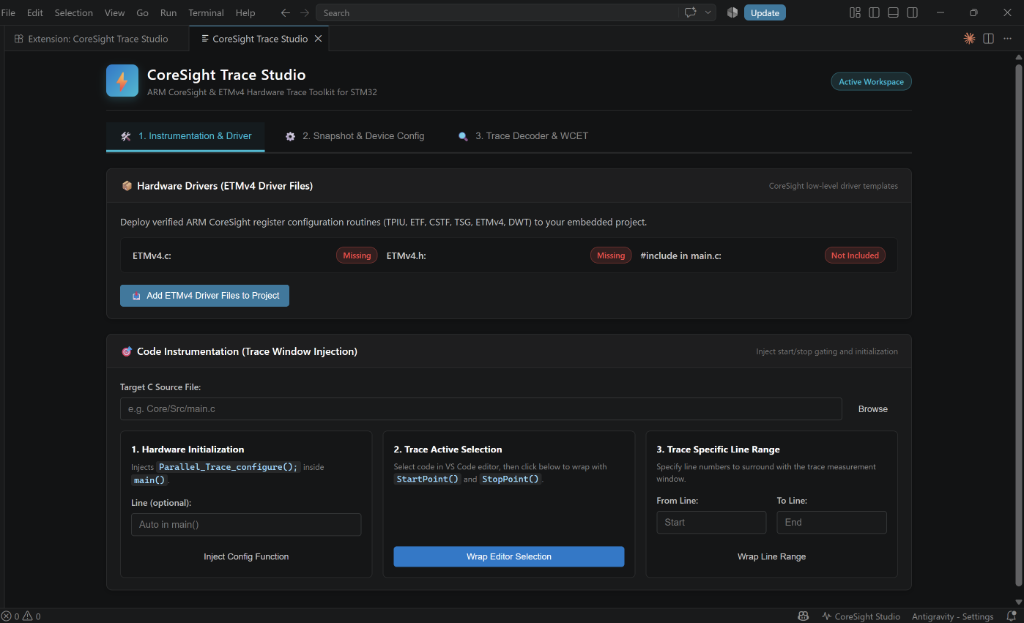
\includegraphics[width=0.95\textwidth]{figures/vscode_tab1_instrumentation.png}
\caption{نمای تب اول افزونه \lr{CoreSight Trace Studio}: مدیریت فایل‌های درایور \lr{ETMv4} و تزریق خودکار پنجره ردیابی}
\label{fig:vscode_tab1}
\end{figure}

\subsection[تب دوم: پیکربندی اسنپ‌شات و ثبّات‌ها]{تب دوم: پیکربندی اسنپ‌شات و ثبّات‌های سخت‌افزاری (\lr{Snapshot \& Device Config})}
تب دوم افزونه (شکل \ref{fig:vscode_tab2}) ارتباط میان خروجی‌های لاجیک‌آنالایزر و دکودر مرجع \lr{OpenCSD} را برقرار می‌سازد:
\begin{enumerate}
    \item \textbf{ورود فایل‌های ثبت سیگنال و باینری (\lr{Capture \& Firmware Files}):} کاربر فایل خروجی نمونه‌برداری لاجیک‌آنالایزر (در قالب فایل متنی \lr{CSV} یا فایل باینری \lr{Wire}) و فایل باینری فریمورک کامپایل‌شده (\lr{.elf}) را انتخاب می‌کند.
    \item \textbf{پیکربندی گرافیکی هسته و ثبّات‌های \lr{ETMv4}:} در این بخش، کاربر پارامترهای پیکربندی را به صورت بصری تعیین می‌نماید:
    \begin{itemize}
        \item \textbf{توصیف پردازنده (\lr{device1.ini}):} مشخص کردن نام و نوع هسته پردازشی (\lr{Cortex-M7}) و آدرس شروع اجرای برنامه (\lr{Initial PC}).
        \item \textbf{تنظیمات ثبّاتی \lr{ETMv4} (\lr{device2.ini}):} تعیین شناسه \lr{Trace ID} گذرگاه \lr{ATB} (مقدار پیش‌فرض ۶۲ معادل \lr{\texttt{0x3E}})، آستانه بسته‌های شمارنده چرخه \lr{TRCCCCTLR} (مقدار پیش‌فرض ۶۴ چرخه)، دوره بسته‌های همگام‌سازی اجباری \lr{TRCSYNCPR} ($2^{10} = 1024$ بایت)، و مد پنجره‌گذاری \lr{ViewInst}.
        \item \textbf{گزینه‌های تکمیلی:} دو چک‌باکس صریح جهت فعال‌سازی درج بسته‌های شمارش چرخه (\lr{CCI / TRCCONFIGR bit 4}) و برچسب زمانی سراسری (\lr{TS / TRCCONFIGR bit 11}).
    \end{itemize}
    با کلیک بر روی دکمه \lr{\texttt{Generate OpenCSD Snapshot Directory}}، پوشه اسنپ‌شات استاندارد شامل فایل‌های \lr{\texttt{snapshot.ini}}، \lr{\texttt{device1.ini}}، \lr{\texttt{device2.ini}}، \lr{\texttt{trace.ini}} و قطعات حافظه فلش به صورت کاملاً همگام و منطبق با کدهای میکروکنترلر ساخته می‌شود.
\end{enumerate}

\begin{figure}[H]
\centering
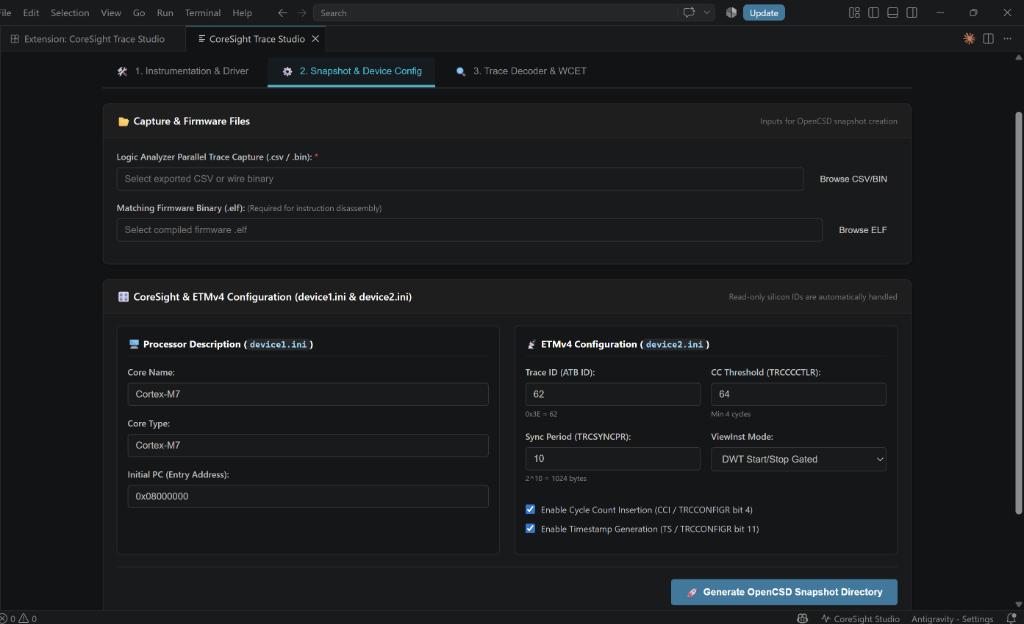
\includegraphics[width=0.95\textwidth]{figures/vscode_tab2_snapshot_config.png}
\caption{نمای تب دوم افزونه \lr{CoreSight Trace Studio}: ورود فایل‌های داده و باینری و تولید متناظر فایل‌های اسنپ‌شات \lr{OpenCSD}}
\label{fig:vscode_tab2}
\end{figure}

\subsection[تب سوم: دکود، استخراج \lr{WCET} و داشبورد]{تب سوم: رمزگشایی، محاسبه \lr{WCET} و داشبورد عملکرد (\lr{Trace Decoder \& WCET})}
تب سوم افزونه (شکل \ref{fig:vscode_tab3}) موتور اجرایی، مرکز محاسبه \lr{WCET} و نمایش گرافیکی نتایج است:
\begin{enumerate}
    \item \textbf{موتور اجرایی رمزگشایی (\lr{Decoder Execution Engine}):}
    \begin{itemize}
        \item دریافت مسیر اسنپ‌شات و باینری \lr{ELF}.
        \item قابلیت انتخاب موتور دکودر پشتیبان بین دکودر پایتون (\lr{\texttt{TempDecoder\_V0.2.py}}) و موتور مرجع \lr{OpenCSD trc\_pkt\_lister}.
        \item دریافت فرکانس ساعت کاری هسته (\lr{Core Clock Frequency}) بر حسب مگاهرتز (مقدار پیش‌فرض ۴۸۰ مگاهرتز برای \lr{STM32H750}). این فرکانس برای تبدیل مستقیم چرخه‌های شمارش‌شده پردازنده به زمان حقیقی اجرای کد به کار می‌رود:
        \begin{equation}
        t_{\mathrm{exec}} = \frac{N_{\mathrm{cycles}}}{f_{\mathrm{core}}}
        \end{equation}
        \item گزینه‌های خط فرمان دکودر شامل دیس‌اسمبل دستورات (\lr{\texttt{-decode}})، پنهان‌سازی بسته‌های خام برای افزایش سرعت (\lr{\texttt{-decode\_only}})، و استخراج آماره‌های تفصیلی عملکرد (\lr{\texttt{-stats}}).
        \item دکمه اجرای پردازش: \lr{\texttt{Run Trace Decoder \& Compute WCET}}.
    \end{itemize}
    \item \textbf{داشبورد شاخص‌های کلیدی عملکرد (\lr{KPI Metrics}):} پس از پایان پردازش، پنج کارت آماری به صورت آنی مقادیر را نمایش می‌دهند:
    \begin{itemize}
        \item \textbf{تعداد دستورات رمزگشایی‌شده (\lr{Instructions Decoded}):} شمار کل دستورالعمل‌های اسمبلی که در طول پنجره ردیابی با موفقیت اجرا و بازسازی شده‌اند.
        \item \textbf{مجموع چرخه‌های ساعت (\lr{Total Clock Cycles}):} تعداد کل پالس‌های کلاک صرف‌شده در اجرای کد بر پایه بسته‌های \lr{CCI}.
        \item \textbf{بیشینه زمان اجرا (\lr{Execution Time / WCET}):} زمان اجرای استخراج‌شده بر حسب میکروثانیه ($\mu\mathrm{s}$) با دقت نانوثانیه‌ای ناشی از شمارش چرخه‌ای.
        \item \textbf{میانگین چرخه‌ها به ازای هر دستور (\lr{Average CPI}):} شاخص کارایی معماری و تأخیر خط‌لوله پردازنده.
        \item \textbf{تعداد تصمیمات انشعاب (\lr{Branch Atoms}):} شمار اتم‌های پرش شرطی (\lr{E/N Atom}) که پیچیدگی مسیرهای اجرایی را مشخص می‌کند.
    \end{itemize}
    \item \textbf{کنسول دکودر و لاگ دیس‌اسمبل (\lr{Decoder Console}):} ترمینال تعبیه‌شده در انتهای صفحه، لاگ خط‌به‌خط دستورات اسمبلی، برچسب‌های زمانی و کدهای وضعیت را همراه با امکان پاک‌سازی سریع به صورت زنده نمایش می‌دهد.
\end{enumerate}

\begin{figure}[H]
\centering
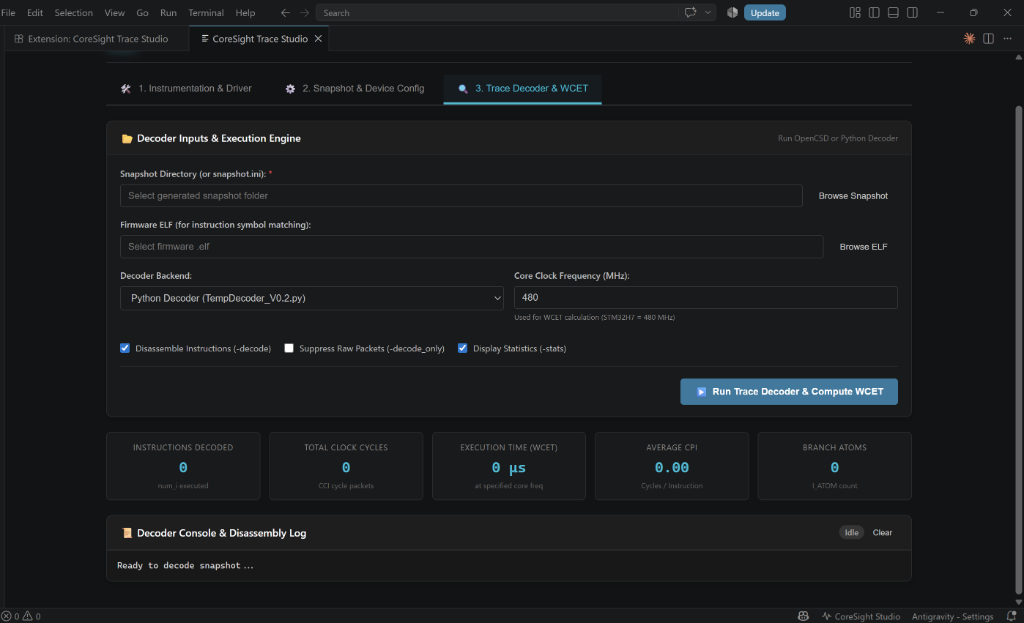
\includegraphics[width=0.95\textwidth]{figures/vscode_tab3_decoder_wcet.png}
\caption{نمای تب سوم افزونه \lr{CoreSight Trace Studio}: موتور پردازش، داشبورد شاخص‌های کلیدی \lr{WCET} و کنسول لاگ دکود}
\label{fig:vscode_tab3}
\end{figure}

\section{جمع‌بندی فصل}
\label{sec:decoding_summary}
در این فصل، معماری کامل اسکریپت پردازش داده‌های ردیابی موسوم به \lr{\texttt{TraceStreamProcessor.py}}، فرآیند آشکارسازی لبه‌ها و بازیابی بایت‌های فریم پورت \lr{TPIU}، اعتبارسنجی یکپارچگی سیگنال‌ها و ادغام با موتور مرجع صنعتی \lr{OpenCSD} مستند گردید. علاوه بر این، کالبدشکافی عمیق فایل‌های اسنپ‌شات ارائه شد و انطباق ضروری پارامترهای دکودر با ثبّات‌های سخت‌افزاری پردازنده تبیین شد. در نهایت، طراحی و پیاده‌سازی افزونه اختصاصی محیط توسعه \lr{VS Code} تحت عنوان \lr{CoreSight Trace Studio} به عنوان یک ابزار جامع سه زبانه تشریح گردید؛ ابزاری که از تزریق خودکار درایورها و پنجره‌های پایش تا تولید هماهنگ اسنپ‌شات و استخراج آماری شاخص‌های \lr{WCET} را به صورت یکپارچه محقق ساخته است. در فصل هفتم، ارزیابی تجربی و صحه‌گذاری آزمایشگاهی این خط‌لوله در سناریوهای آزمون واقعی مورد بررسی قرار خواهد گرفت.
